\chapter{Felhasználói dokumentáció}
\label{ch:user}

\section{Rendszerkövetelmények}

\subsection{Futtatás}

Magának webalkalmazás szerveroldalának a futtatásához a ASP.NET Core Runtime 8.0-ra van szükség, amelyhez
szükséges az alábbi operációs rendszerek valamelyike:
\begin{compactitem}
	\item Windows 10, 11 vagy Server 2012+
	\item 64-bites Ubuntu 20.04+ vagy Debian 11+
	\item macOS 10.15+ (csak külső, hosztolt szerver esetén támogatott)
\end{compactitem} 
A memóriahasználat a felhasználóktól nagyban függ, így 0,5 GB-tól akár 4 GB RAM-ra is szüksége lehet a szervernek a zökkenőmentes futáshoz. A merevlemezen történő tárhelyhasználat nagyban függ az éppen bejelentett pontok méretétől és legfőképp az azokhoz csatolt fényképektől. Magához a futtatáshoz elegendő 0,5 GB tárhely is (az ehhez szükséges szoftvereket nem bele értve), viszont az alkalmazás használtat közben ez nagy mértékben fog növekedni az előbb említett okok miatt, így érdemes akár saját, nagy kapacitású merevlemezre telepíteni a szerveroldalt.
Az szerver által használt SQL Server adatbázishoz (későbbiekben MSSQL-adatbázis) a Microsoft SQL Server szoftver valamelyik, de lehetőség szerint a legfrissebb, 2019-es verziójára van szükség, melyet a fentebb említett operációs rendszerek bármelyike képes futtatni.
Az első üzembe helyezést követően nincsen szükség további rendszergazdai feladatokra.
\subsection{Használat}

A program felhasználói felülete egy weboldal. Ennek meglátogatásához elsősorban szükség van egy olyan operációs rendszer telepítésére, majd futtatására, melyre elérhető bármilyen friss, Chromium-alapú webböngésző. Egy ilyen böngésző a Google Chrome, amellyel ajánlott a weboldal látogatása. Hardver- és szoftver követelményei az alábbiak:
\begin{compactitem}
	\item Operációs rendszerek valamelyike:
	\begin{compactitem}
		\item Windows 10, 11 vagy Server 2012+
		\item 64-bites Ubuntu 20.04+ vagy Debian 11+
		\item macOS 10.15+
		\item Android 8.0+ vagy Chrome OS
	\end{compactitem}
	\item Minimális hardver követelmények:
	\begin{compactitem}
		\item Pentium 4+ (vagy más, SSE3-at támogató) processzor
		\item 2 (ajánlottan 4) GB RAM
	\end{compactitem}
\end{compactitem}

Felhasználóként első üzembe helyezésre nincsen szükség, elég ha a felhasználó meglátogatja az oldalt. Ha még nem regisztrált felhasználói fiókot, akkor bizonyos funkciók eléréséhez regisztrálnia kell.

\section{Általános felhasználói tájékoztató}

Az weboldal használtat közben négy felhasználói típusról beszélhetünk: vendég, regisztrált (és bejelentkezett) felhasználó, moderátor és adminisztrátor. Így vendégnek számít aki még nem regisztrált, vagy ha igen, akkor nem jelentkezett be fiókjával, moderátornak aki moderátori szintű fiókkal és adminisztrátornak, aki adminisztrátori szintű fiókkal azonosította magát a bejelentkező felületen.
\newpage

\section{Funkciók vendégként}

\noindent Egy vendég felhasználó számára hat funkció érhető el a weboldalon:
\begin{compactitem}
	\item regisztrálás új-, illetve bejelentkezés már meglévő fiókba
	\item a térkép megtekintése a bejelentett pontokkal (ez a főoldal)
	\item egy-egy pont adatainak részletesebb megtekintése
	\item az összes pont listázása
	\item a weboldal színsémájának ("sötét"- vagy "világos" mód) tetszőleges beállítása
\end{compactitem}

\begin{figure}[H]
	\centering
	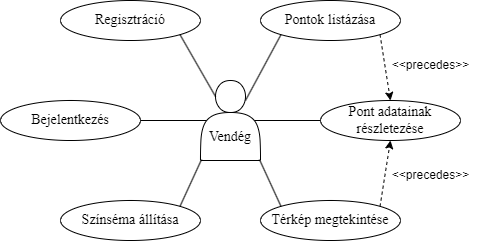
\includegraphics[width=0.6\textwidth]{usecase_guest}
	\caption{Felhasználói esetek vendégként}
	\label{fig:usecase_guest}
\end{figure}

\subsection{Felület áttekintése}
\label{subsec:nav_guest}

A weboldal látogatása során több felület is megjelenik, viszont ezek általánosan leírhatóak. Minden lap tetején egy navigációs sáv van, melynek segítségével több funkciót is gyorsan elérhetünk. A sáv bal oldalán a weboldal neve, illetve a "Térkép" felirat egyaránt a térképre, azaz a főoldalra irányít, a mellette szereplő "Lista" pedig a pontok listájához. A másik oldalon (jobbról balra) egy fizikai kapcsolót imitáló gomb, melynek segítségével válthatunk az előbb említett színsémák között, illetve amellett egy "Nincs bejelentkezve" feliratú listát lenyitva tudunk a regisztráció, illetve a bejelentkezés közül választani.\par
Ha a felhasználó nem egy széles képernyőn (pl. asztali számítógép vagy fektetett táblagép) látogatja meg az oldalt, akkor a sáv bár hasonlóan ott van, viszont a könnyebb használat érdekében a menüpontok egy, a jobb oldalon található \hspace{0.1cm}\boldmath\(\equiv\)\hspace{0.1cm} ikonra kattintva lehet ezeket elérni.

\begin{figure}[H]
	\centering
	\subcaptionbox{Nagy méretű kijelző}{
		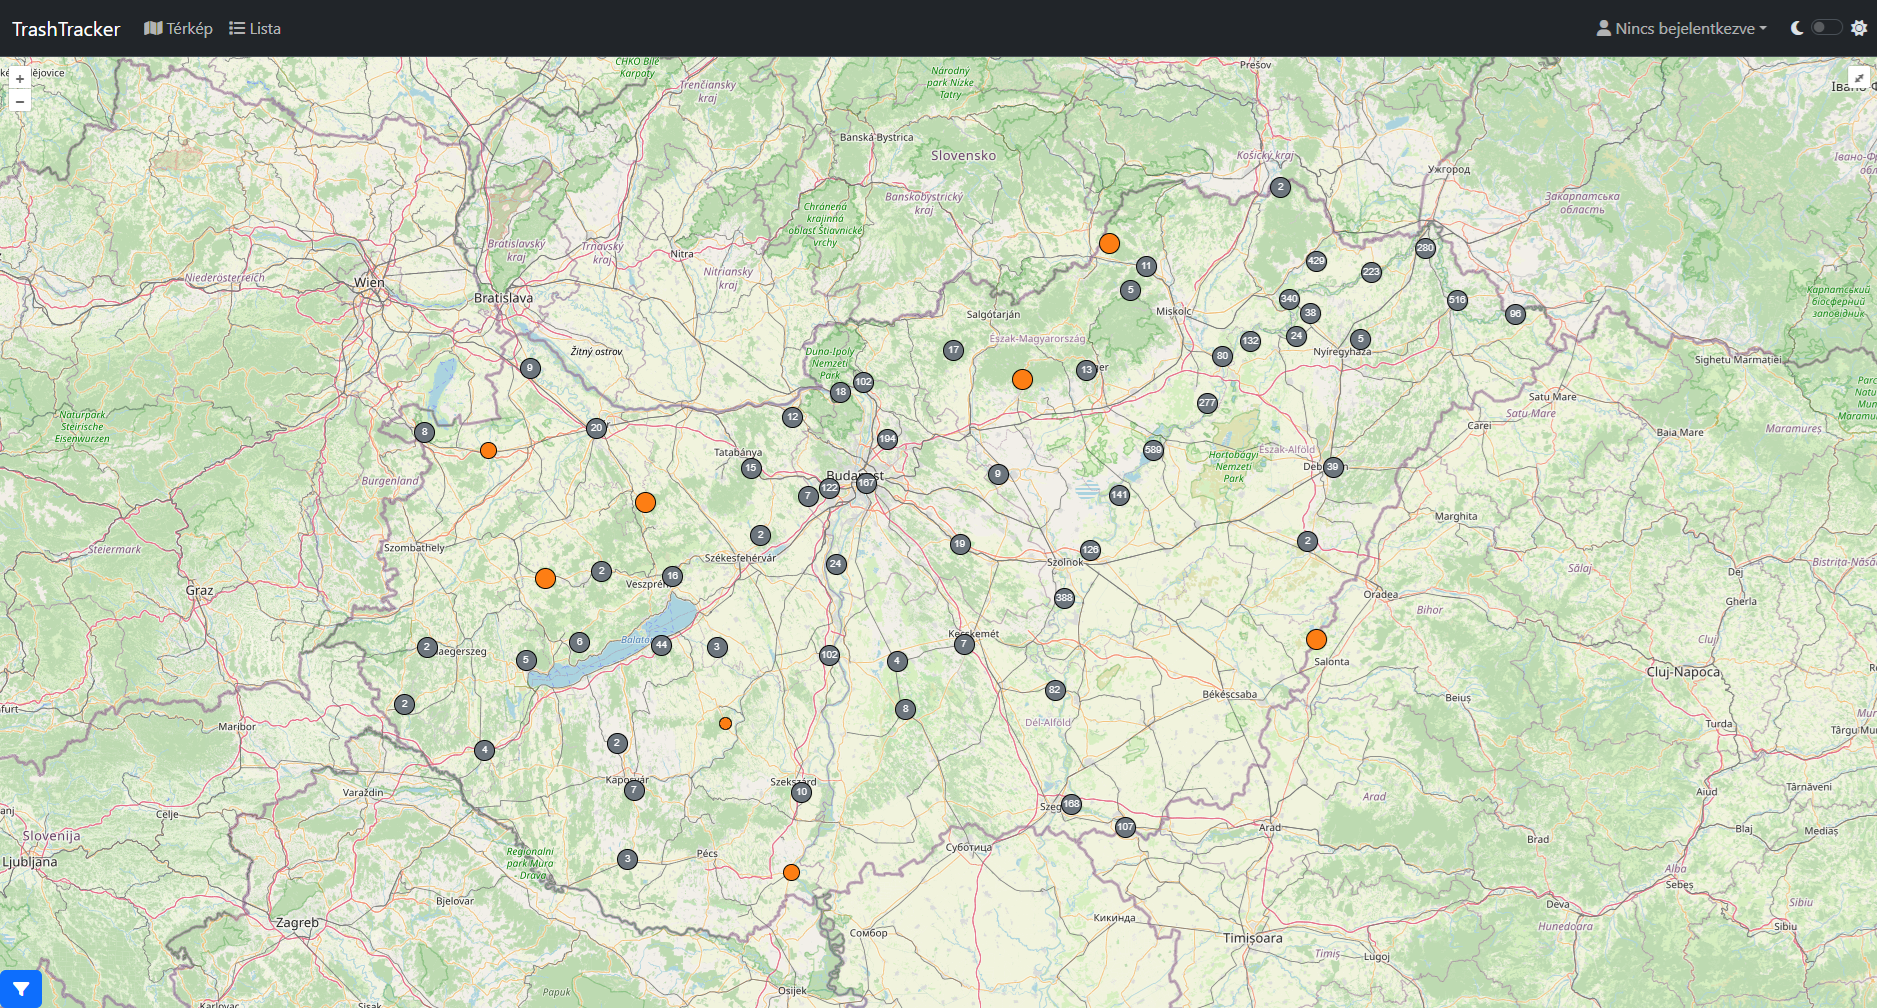
\includegraphics[width=0.45\linewidth]{map}}
	\hspace{5pt}
	\subcaptionbox{Kis méretű kijelző}{
		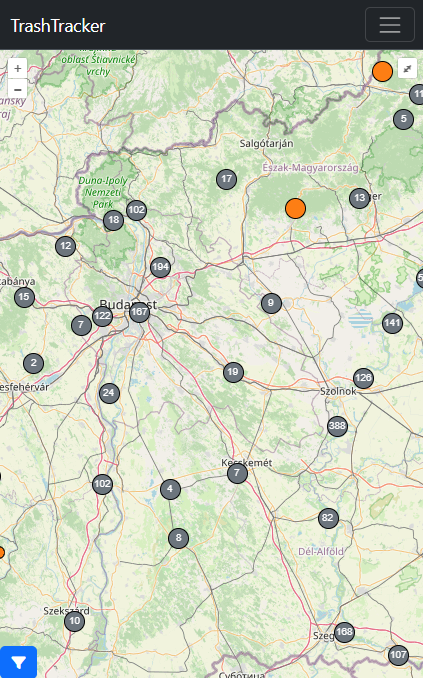
\includegraphics[width=0.2\linewidth]{map_phone}}
		\hspace{5pt}
	\subcaptionbox{Kis méretű kijelző (lenyitott navigációs sávval)}{
		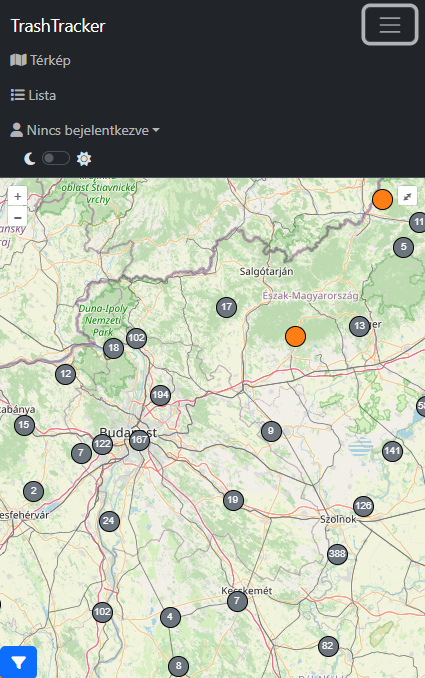
\includegraphics[width=0.2\linewidth]{map_phone_menu}}
	\caption{A felület kinézete a kezdőoldalon különböző méretű kijelzők esetén}
	\label{fig:map_guest}
\end{figure}

\subsection{Térkép (kezdőoldal)}

A navigációs sávon a weboldal nevére, illetve a "Térkép" feliratra kattintva azonnal a bejelentett pontok térképére navigálhatunk. Ennek kezelése a már jól ismert térképes alkalmazásokéhoz hasonló. A bal felső sarokban található \hspace{0.1cm}\boldmath\(+\)\hspace{0.1cm}, illetve \hspace{0.1cm}\boldmath\(-\)\hspace{0.1cm} ikonra kattintva nagyítani, illetve kicsinyíteni lehet, emellett egérrel a görgő görgetésével és érintőképernyőn két ujj összehúzásával/széttolásával is lehetőség van. A jobb felső sarokban a térképet teljes képernyős módba is lehet helyezni, melynek ismételt megnyomásával, vagy billentyűzeten az Esc gombbal ki lehet lépni. A bal alsó sarokban található a szűrés gomb, melynek segítségével különböző, a felhasználók által jelentett tulajdonságok szerint van lehetőség.

\subsubsection{Jelmagyarázat}

A térképen a pontok különböző mérettel és színnel jelennek meg, melyeknek céljuk a fontosabb információk lehetőség szerinti kiemelése.\\
A szemét mennyisége szerint a pont mérete lehet
\begin{compactitem}
	\item[\large\textbullet] kicsi (8 pixel), azaz "elfér egy zsákban",
	\item[\Large\textbullet] közepes (10 pixel), azaz "elfér egy talicskában" és
	\item[\LARGE\textbullet] nagy (12 pixel), azaz "autóra van szükség".
\end{compactitem}\newpage
A szemét első bejelentés óta levő állapota szerint a pont színe lehet
\begin{compactitem}
	\item[\textcolor{tt_green}{\Large\textbullet}] zöld, azaz "megtisztítva",
	\item[\textcolor{tt_yellow}{\Large\textbullet}] sárga, azaz "kevesebb",
	\item[\textcolor{tt_orange}{\Large\textbullet}] narancs, azaz "még mindig itt van" és
	\item[\textcolor{tt_red}{\Large\textbullet}] piros, azaz "több".
\end{compactitem}

\subsubsection{Szűrés}

A fentebb említett szűrés gombra kattintva a képernyő alján beúszik egy görgethető menü, amely a pontok tulajdonságai szerinti szűrést teszi lehetővé. A szemét mennyisége és állapota mellett annak típusa és hozzáférhetősége szerint is lehet válogatni. Ezeket a beúszó menün található, tulajdonságok szerint csoportosított "kapcsoló" gombokkal lehet elérni. Ha egy ilyen gomb kék színű, akkor igen, ha átlátszó, akkor pedig nem szeretnénk a térképen látni. Alapértelmezetten az összes ilyen gomb "igen" állapotban van. A gombok között szűrés esetén a logikai vagy művelete értelmezett, tehát ha bejelölésre kerül egy tulajdonság, viszont egy másik nem, akkor attól függetlenül a bejelöletlen attribútum még előfordulhat a megjelenített pontok között, feltéve, hogy legalább egy bejelölt jellemzővel rendelkezik. Ezt a menüt a jobb felső sarokban található \hspace{0.1cm}\boldmath\(\times\)\hspace{0.1cm} gombra nyomva lehet bezárni, a szűrőket megtartva, egy másik oldalra navigálásig vagy az oldal újratöltéséig.

\begin{figure}[H]
	\centering
	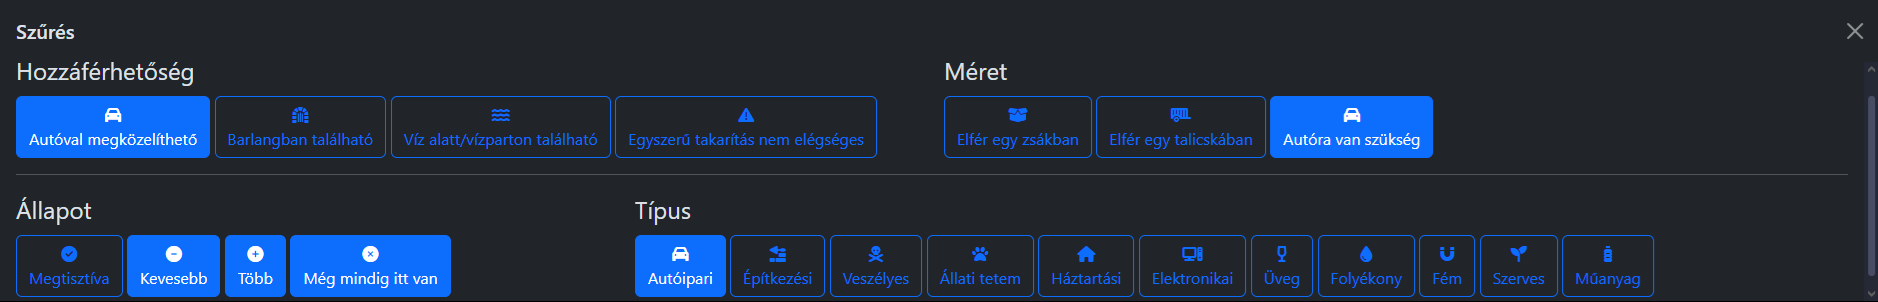
\includegraphics[width=1\textwidth]{map_filter}
	\caption{A kezdőoldal alján beúszó szűrési menü}
	\label{fig:map_filter}
\end{figure}

\subsubsection{Betekintés és részletek}

Egy pontra való kattintáskor afelett megjelenik egy modális "buborék", amely minimális információt és egy képet tartalmaz a hozzátartozó szemétről. Emellett a kis ablak alján található egy "Részletek" gomb, melyre kattintva elnavigálhatunk az azt részletező adatlapra.

\begin{figure}[H]
	\centering
	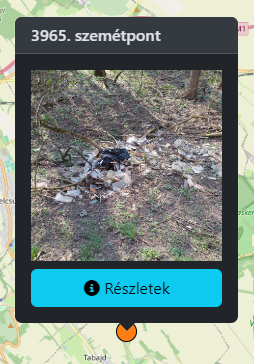
\includegraphics[width=0.225\textwidth]{map_popover}
	\caption{Példa egy felbukkanó buborékra egy ponton}
	\label{fig:map_popover}
\end{figure}

\subsection{Pont részletezése}
\label{subsec:trash_details}

Ezt az oldalt az előző bekezdésben említett "Részletek" gombra kattintva, vagy a következő bekezdésben tárgyalt \faIcon{info-circle} ikonra kattintva lehet elérni. Itt az egyszerű tulajdonságok részletezésén túl megtalálható a pont pontos helyzete, illetve annak forrása (felhasználó esetén bejelentője). Előbbire kattintva a térképen levő helyére, utóbbira pedig annak forrására (TrashOut esetén az ottani adatlapjára, felhasználó esetén annak a profiljára) lehet navigálni.

\begin{figure}[H]
	\centering
	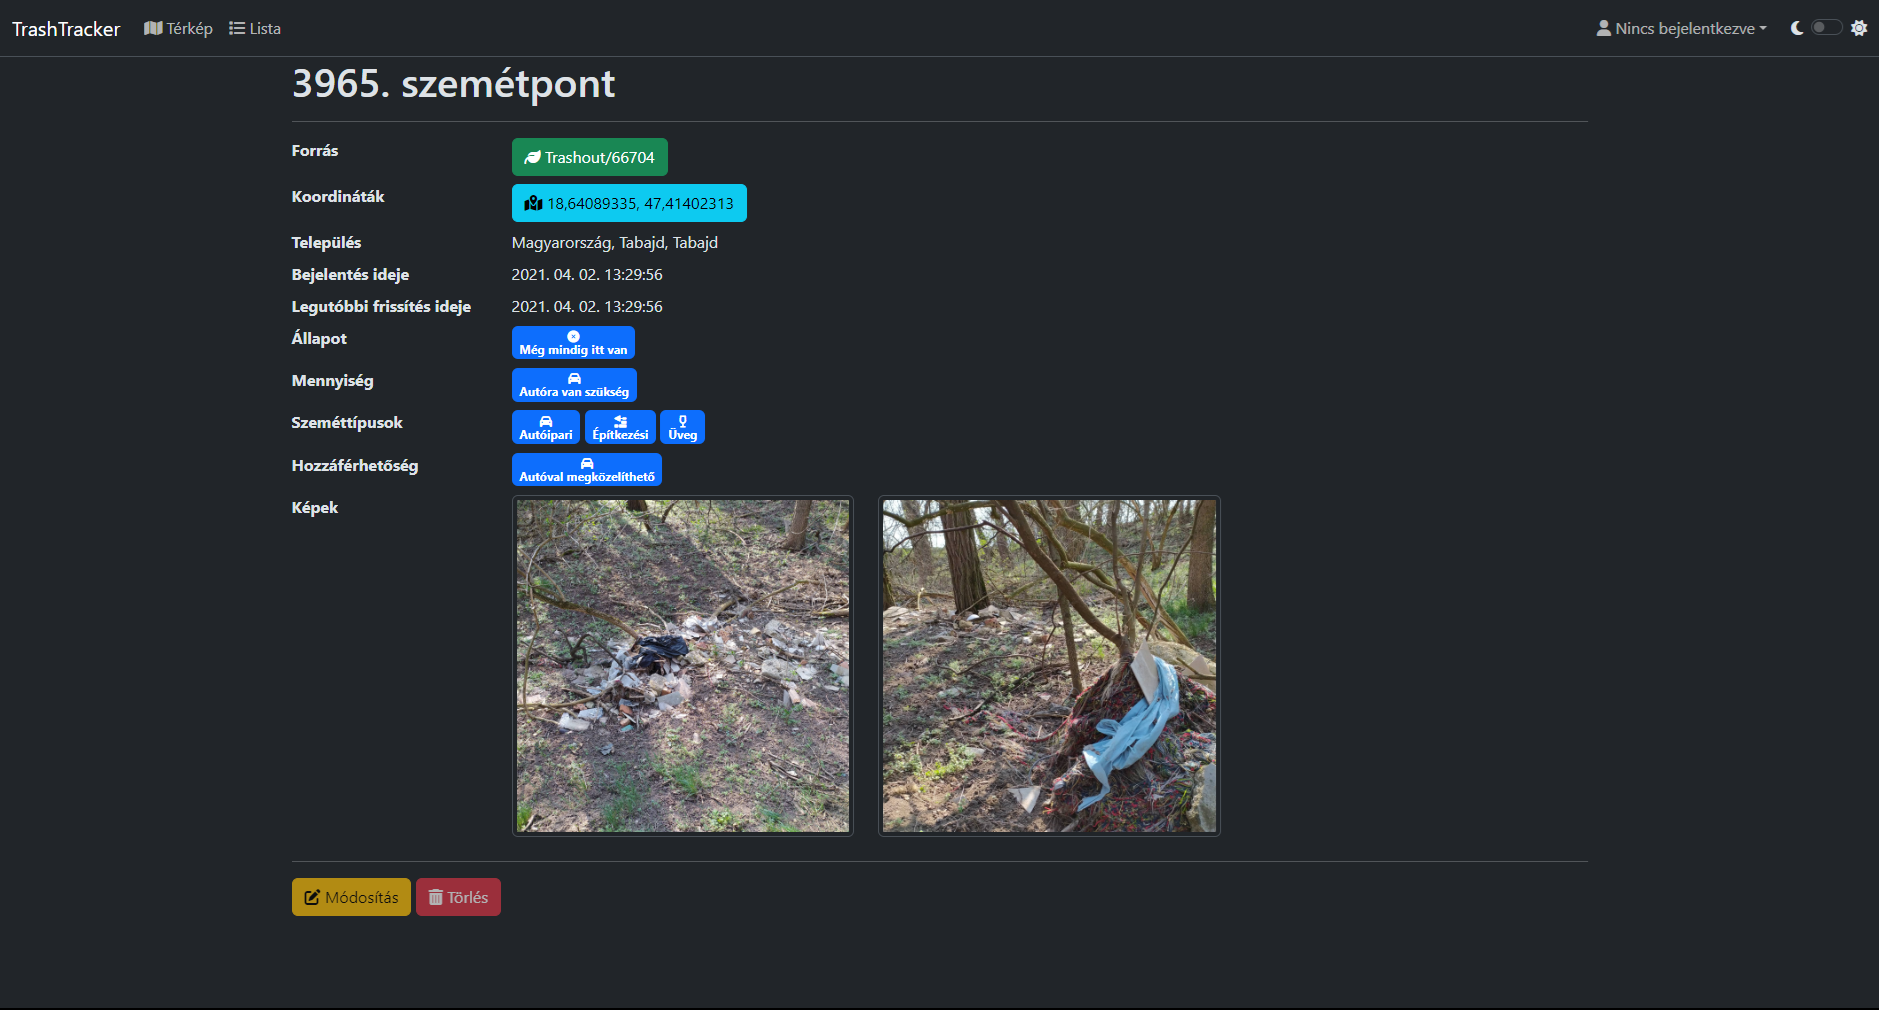
\includegraphics[width=0.7\textwidth]{trash_details}
	\caption{Példa egy szemétpontot részletező adatlapra}
	\label{fig:trash_details}
\end{figure}

\subsection{Listanézet}
\label{subsec:trash_index}

A pontokat nem csak térképen, hanem listaként is megtekinthetjük. Ennek célja, hogy a bejelentés/frissítés dátuma szerint rendezve könnyedén fel lehessen fedezni a legrelevánsabb szemétlerakatokat. A lista minden sora egy-egy pontot, annak oszlopai pedig annak a fejlécben szereplő tulajdonságát tartalmazzák. Egy adott rekord részletezésére is lehetőség van, a jobb oldalon található \faIcon{info-circle} ikonra kattintva. Az oldal tetején lehetőség van alapvető szűrésekre is, opcionálisan belefoghatjuk a listába a már megtisztított pontokat, kereshetünk a bejelentő felhasználónevében, illetve az ahhoz tartozó megjegyzéseiben, illetve állíthatjuk az egy oldalon szereplő találatok maximális számát. Ha több találat van, mint ami az oldalon elfér, akkor a lista tetején, illetve alján található nyilakkal és számokkal könnyedén navigálhatunk azok között.

\begin{figure}[H]
	\centering
	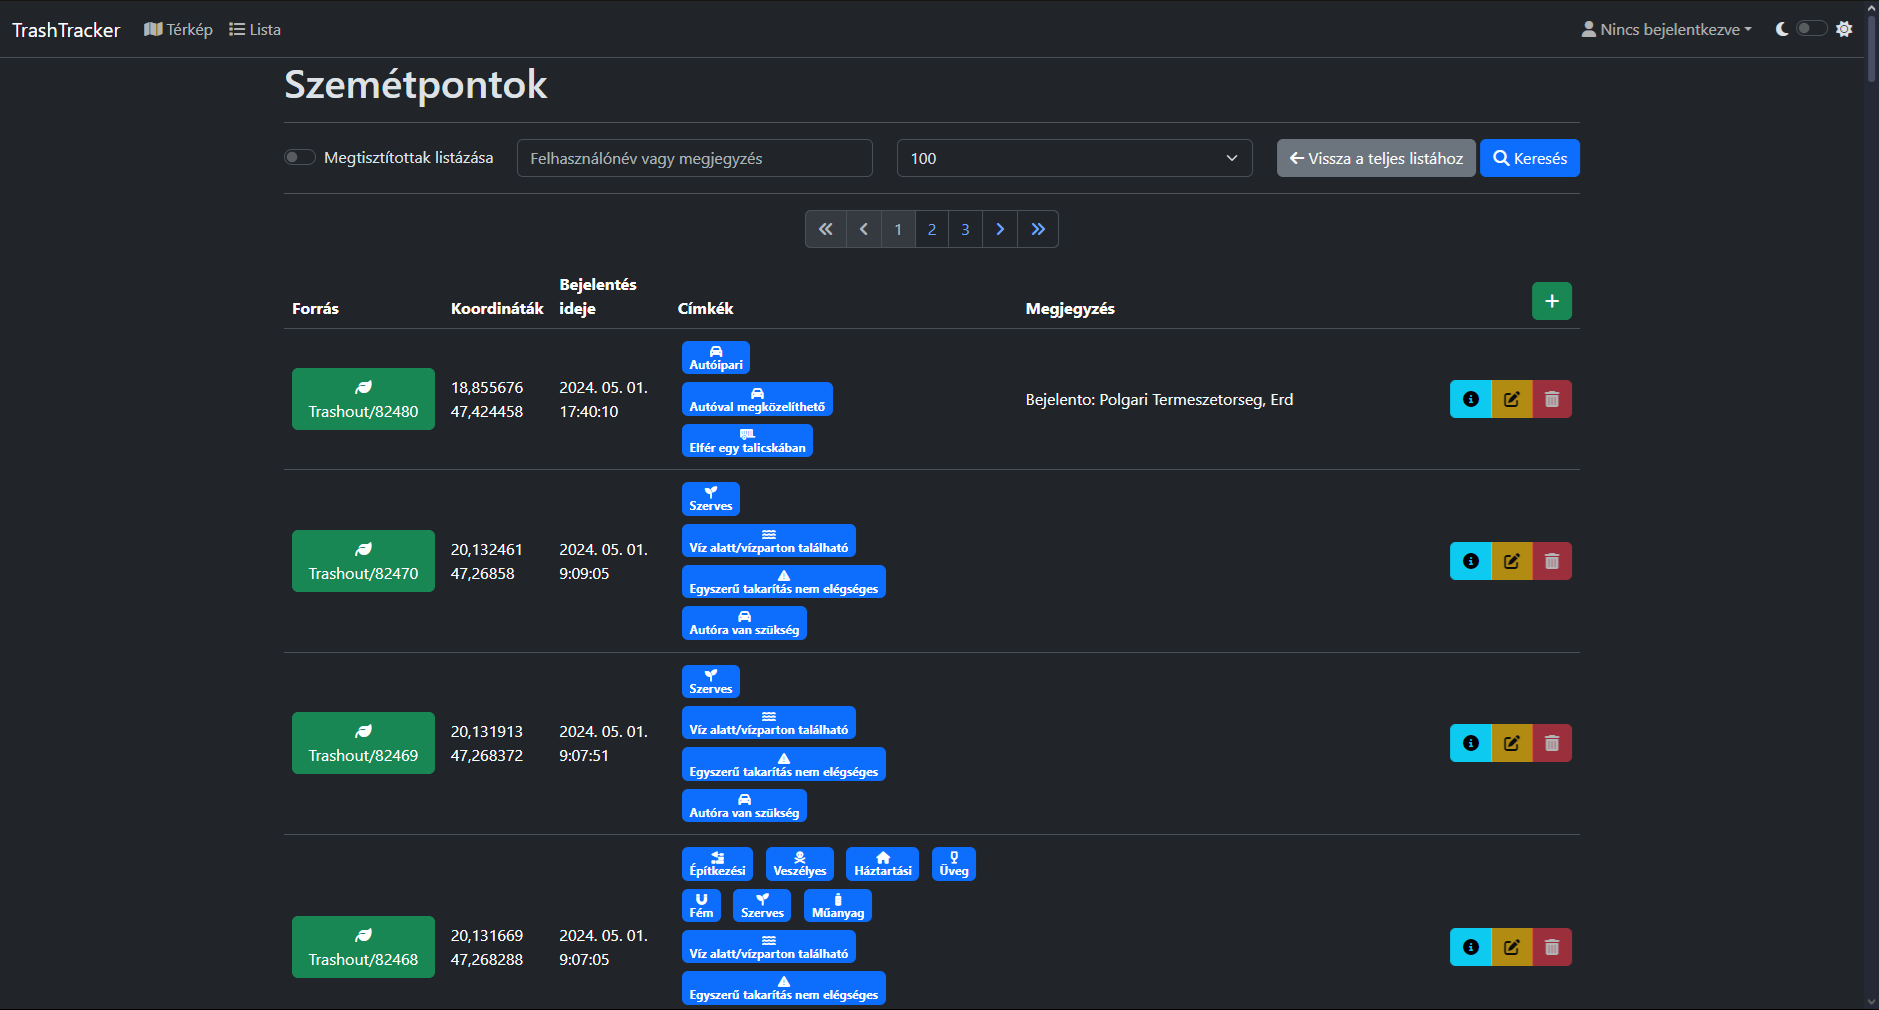
\includegraphics[width=0.7\textwidth]{trash_index}
	\caption{Szemétpontok listanézetének felülete}
	\label{fig:trash_index}
\end{figure}


\subsection{Színséma választása}

Minden oldal navigációs sávjának jobb szélén található egy kapcsoló mellyel könnyedén állítható az adott oldal színsémája, melynek bal- (\faIcon{moon}) állása sötét, illetve jobb oldali (\faIcon{sun}) állása világos módot jelent. Alapértelmezetten ez az előbbi állapotban van az energiatakarékosabb működés és a szemet jobban kímélő megjelenés miatt. Ez a beállítás szabadon állítható, mely megmarad minden aloldalon a böngészés idejére.

\begin{figure}[H]
	\centering
	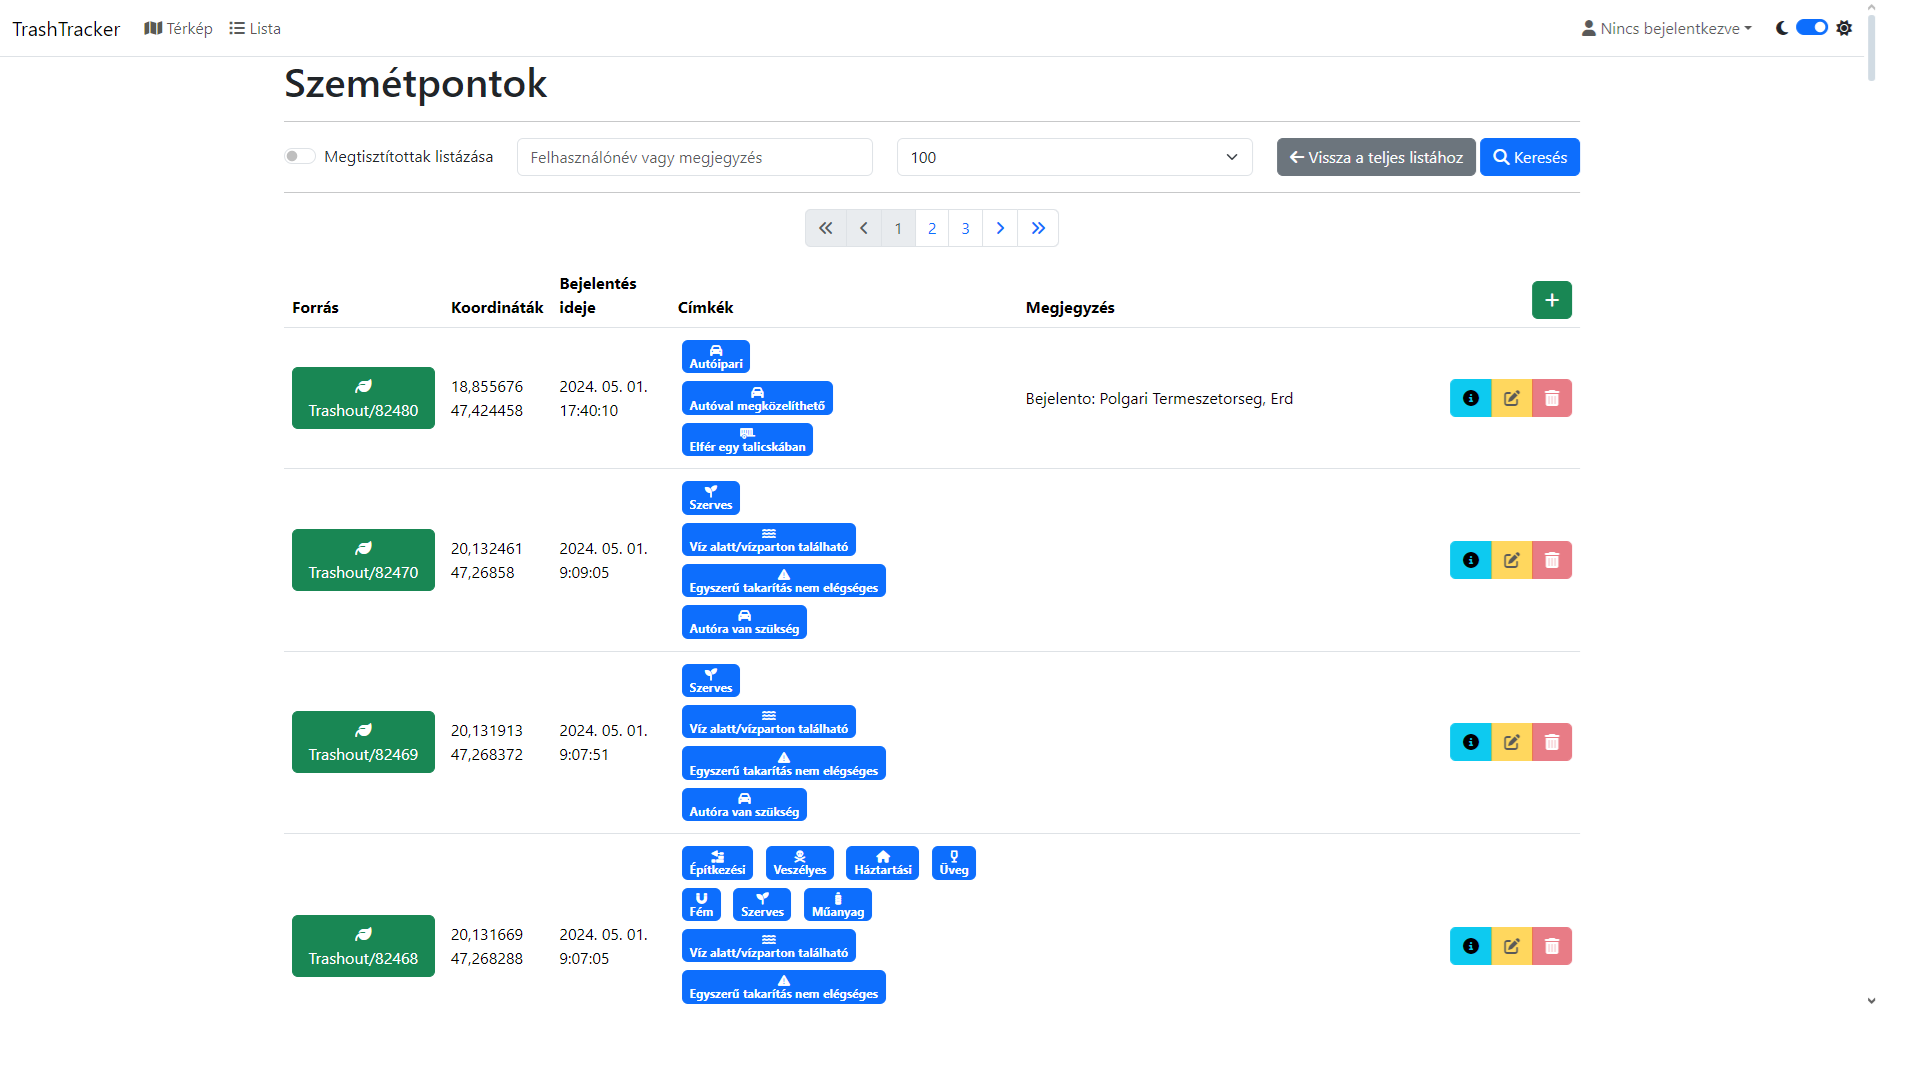
\includegraphics[width=0.7\textwidth]{trash_index_light}
	\caption{Szemétpontok listanézetének felülete világos módban}
	\label{fig:trash_index_light}
\end{figure}

\subsection{Regisztráció}

További funkciók használatáért (pontok bejelentése és frissítése) a felhasználónak egy felhasználói fiókra van szüksége, mely utóbbija ha nincs, akkor regisztrálnia kell hozzá. Ezt a navigációs sáv jobb oldalán található "Nincs bejelentkezve" feliratra kattintva lenyíló menüben szereplő "Regisztráció" menüpontra nyomva érheti el. Ha az előbbi helyett egy \faIcon{user} ikonnal társulva egy felhasználó neve szerepel, akkor az már be van jelentkezve, ezzel kapcsolatosan nincsen teendője.\par
A regisztrációs felületen egy űrlap található, ahol meg kell adni a kívánt felhasználónevet, e-mail címet (elérhetőségként), jelszavat, illetve opcionálisan egy profilképet. Az adatok kitöltése után az űrlap alján található "Regisztráció" gombra kattintva lehet beadni az adatokat, melyek ha megfelelnek a követelményeknek, akkor a felhasználó a főoldalon találja magát, az új fiókjával bejelentkezve.

\begin{figure}[H]
	\centering
	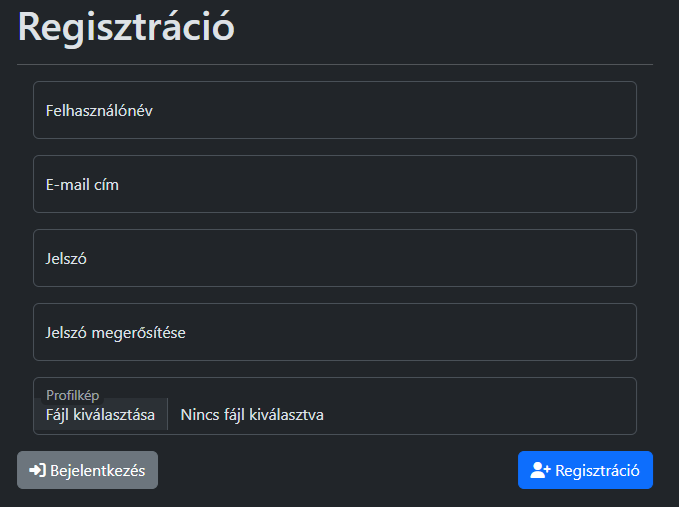
\includegraphics[width=0.7\textwidth]{register_form}
	\caption{A regisztrációs felület űrlapja}
	\label{fig:register_form}
\end{figure}

\subsubsection{Hibaüzenetek}
\label{subsubsec:user_register_errors}

A regisztrációkor megadott adatok több követelménynek is meg kell hogy feleljenek, melyek "megsértésekor" hibaüzenetek jelenhetnek meg az űrlap kitöltése közben vagy után. Az első ilyen követelmény, hogy minden felhasználónévnek egyedinek kell lennie. Ezt az űrlap helyes kitöltése és elküldése után egy "\textcolor{red}{Ez a felhasználónév már foglalt!}" felirat jelzi.

\begin{figure}[H]
	\centering
	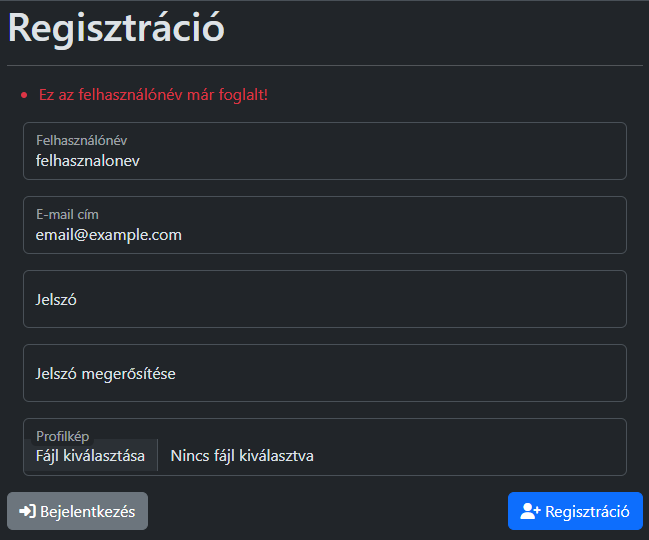
\includegraphics[width=0.7\textwidth]{register_form_duplicate_username}
	\caption{Már foglalt felhasználónév esetén megjelenő hibaüzenet}
	\label{fig:register_form_duplicate_username}
\end{figure}

Ha a megadott e-mail cím nem érvényes (azaz nem felel meg annak formai követelményeihez, pl. legyen benne "@" és egy "."), azt az űrlap kitöltése közben jelzi egy "\textcolor{red}{Érvénytelen e-mail cím!}" feliratú üzenet.

\begin{figure}[H]
	\centering
	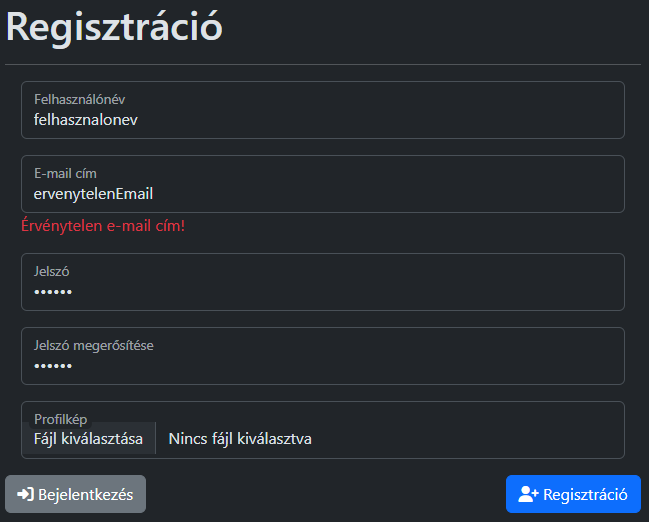
\includegraphics[width=0.7\textwidth]{register_form_invalid_email}
	\caption{Érvénytelen e-mail cím esetén megjelenő hibaüzenet}
	\label{fig:register_form_invalid_email}
\end{figure}

A legtöbb követelmény a jelszavakat érinti, itt több hibaüzenettel is találkozhat a felhasználó. Biztonsági okokból, egy jelszó 6-32 db karakterből kell álljon, melynek tartalmaznia kell legalább egy-egy kis- és nagybetűt, illetve számjegyet is. Ha ennek mégsem felelne meg a megadott jelszó, akkor azt az e-mail címhez hasonlóan egy "\textcolor{red}{A jelszó nem lehet rövidebb 6 és hosszabb 32 karakternél!}" vagy "\textcolor{red}{Jelszónak tartalmaznia kell legalább egy kis- és nagybetűt illetve számjegyet!}" üzenet jelenik meg, annak függvényében, hogy melyik pontján nem megy át az ellenőrzésen (tehát ha túl rövid a jelszó és pl. nem tartalmaz nagybetűt, akkor csak az előbbi jelenik meg, az utóbbi csak ha a hossz javítása után sem felel meg). Emellett a jelszó megerősítésére is szükség van, azaz meg kell adni a beírt jelszót egy második alkalommal is. Ha ezek nem egyeznének meg, azt is egy hibaüzenet jelzi a felhasználó számára.

\begin{figure}[H]
	\centering
	\subcaptionbox{Nem megfelelő hosszú jelszó hibaüzenete}{
		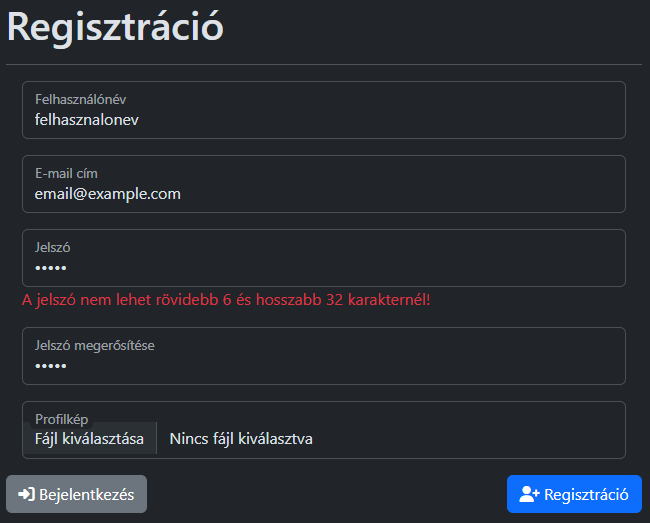
\includegraphics[width=0.3\linewidth]{register_form_invalid_password_length}}
	\hspace{5pt}
	\subcaptionbox{Nem megfelelő karaktereket tartalmazó jelszó hibaüzenete}{
		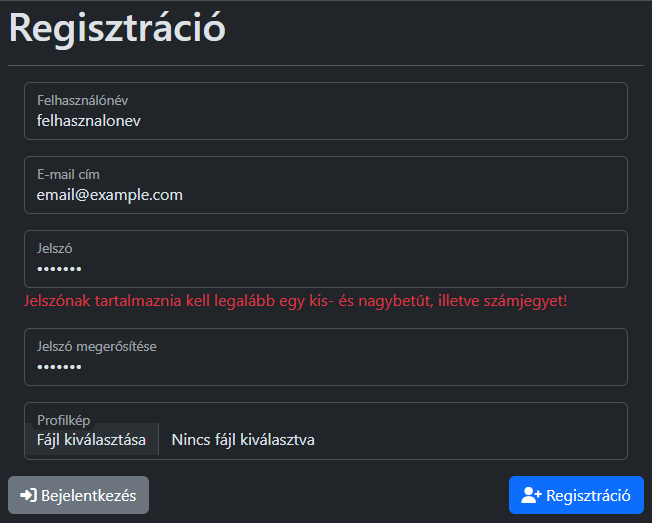
\includegraphics[width=0.3\linewidth]{register_form_invalid_password_characters}}
	\hspace{5pt}
	\subcaptionbox{Nem azonos jelszavak hibaüzenete}{
		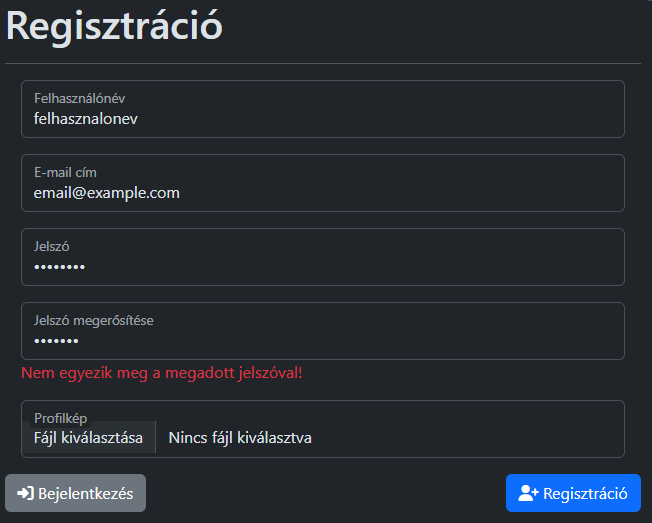
\includegraphics[width=0.3\linewidth]{register_form_invalid_password_repeat}}
	\caption{Érvénytelen jelszó esetén megjelenő hibaüzenetek}
	\label{fig:register_form_invalid_password}
\end{figure}

\subsection{Bejelentkezés}

Ha a felhasználónak már van saját fiókja, akkor ismételt regisztráció helyett beléphet abba, az előző bekezdésben tárgyaltak szerint a "Bejelentkezés" gombra kattintva. Az űrlap hasonló, viszont itt elég csak a felhasználónév (vagy e-mail cím tetszőlegesen), illetve a hozzátartozó jelszó egyszeri megadására. Ha az adatok egyeznek a regisztrációkor megadottakkal, akkor az űrlap alján található "Bejelentkezés" gombra kattintva a felhasználó a főoldalra lesz átirányítva, a felhasználói fiókjába bejelentkezve. Ellenben, ha nem jár sikerrel, akkor üzenetek tájékoztatják a klienst erről. Ha többszöri próbálkozásra sem jár sikerrel, akkor lehetősége van bejelentkezés helyett újabb felhasználó regisztrálására, vagy egy adminisztrátort megkérve bejelentkezési adatainak megváltoztatására is.

\begin{figure}[H]
	\centering
	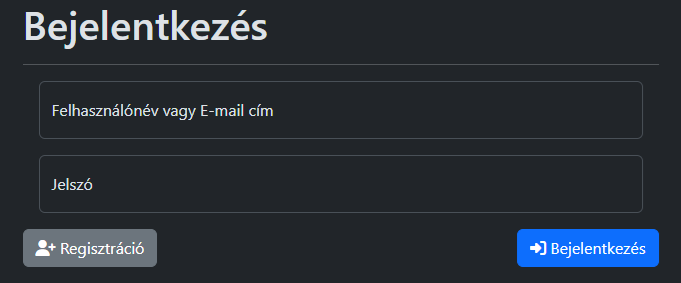
\includegraphics[width=0.7\textwidth]{login_form}
	\caption{A bejelentkezéses felület űrlapja}
	\label{fig:login_form}
\end{figure}

\subsubsection{Hibaüzenetek}

Sikertelen bejelentkezés esetén, azaz nem megfelelő felhasználónév (vagy e-mail cím) és jelszó páros megadásakor biztonsági okok miatt csak egy, a regisztráláskor látottaknál általánosabb "\textcolor{red}{Sikertelen bejelentkezés!}" felirat szerepel.

\begin{figure}[H]
	\centering
	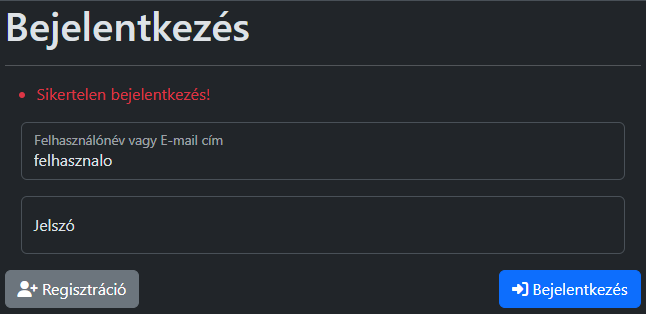
\includegraphics[width=0.7\textwidth]{login_form_error}
	\caption{A bejelentkezéses felület űrlapján szereplő hibaüzenet}
	\label{fig:login_form_error}
\end{figure}

\section{Funkciók felhasználóként}

Sikeres bejelentkezést (vagy regisztrációt) követően a felhasználó vendég helyett bejelentkezett felhasználónak (vagy fióktípusának megfelelőnek) számít. Ezzel további funkciók válnak elérhetővé, mint például a szemétpontok bejelentése és frissítése, illetve a saját felhasználói fiók profiljának szerkesztése.

\begin{figure}[H]
	\centering
	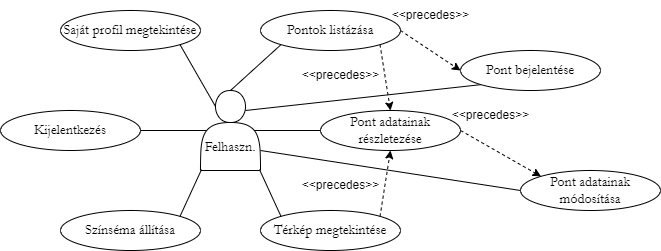
\includegraphics[width=1.0\textwidth]{usecase_user}
	\caption{Felhasználói esetek (bejelentkezett) felhasználóként}
	\label{fig:usecase_user}
\end{figure}

\subsection{Pont bejelentése}

Új pont bejelentésére a listanézet tetején található \faIcon{plus} ikonra kattintva van lehetőség, mely elnavigál annak az űrlapjára. Ezen az űrlapon meg kell adni a szemét pontos helyzetét koordinátákként, amely megadásának segítségül szolgál a szöveges mezőjük melletti "Jelenlegi hely meghatározása", mely megnyomásával a böngésző meghatározza a bejelentőnek a lehető legpontosabb koordinátáit. A méret jellemzése mellett ajánlott a szemét típusát és hozzáférhetőségét is megadni, melynek kezelése hasonló a térképen való szűrés gombjaihoz. Az utolsó, többsoros szöveges mezőben megjegyzést lehet írni, mely segíti a listanézetben való keresését a pontnak. Az űrlap alján a "Vissza" gombbal lehet az előbb meglátogatott oldalra navigálni, illetve a "Bejelentés" gombra kattintva is ide lesz átirányítva a felhasználó

\begin{figure}[H]
	\centering
	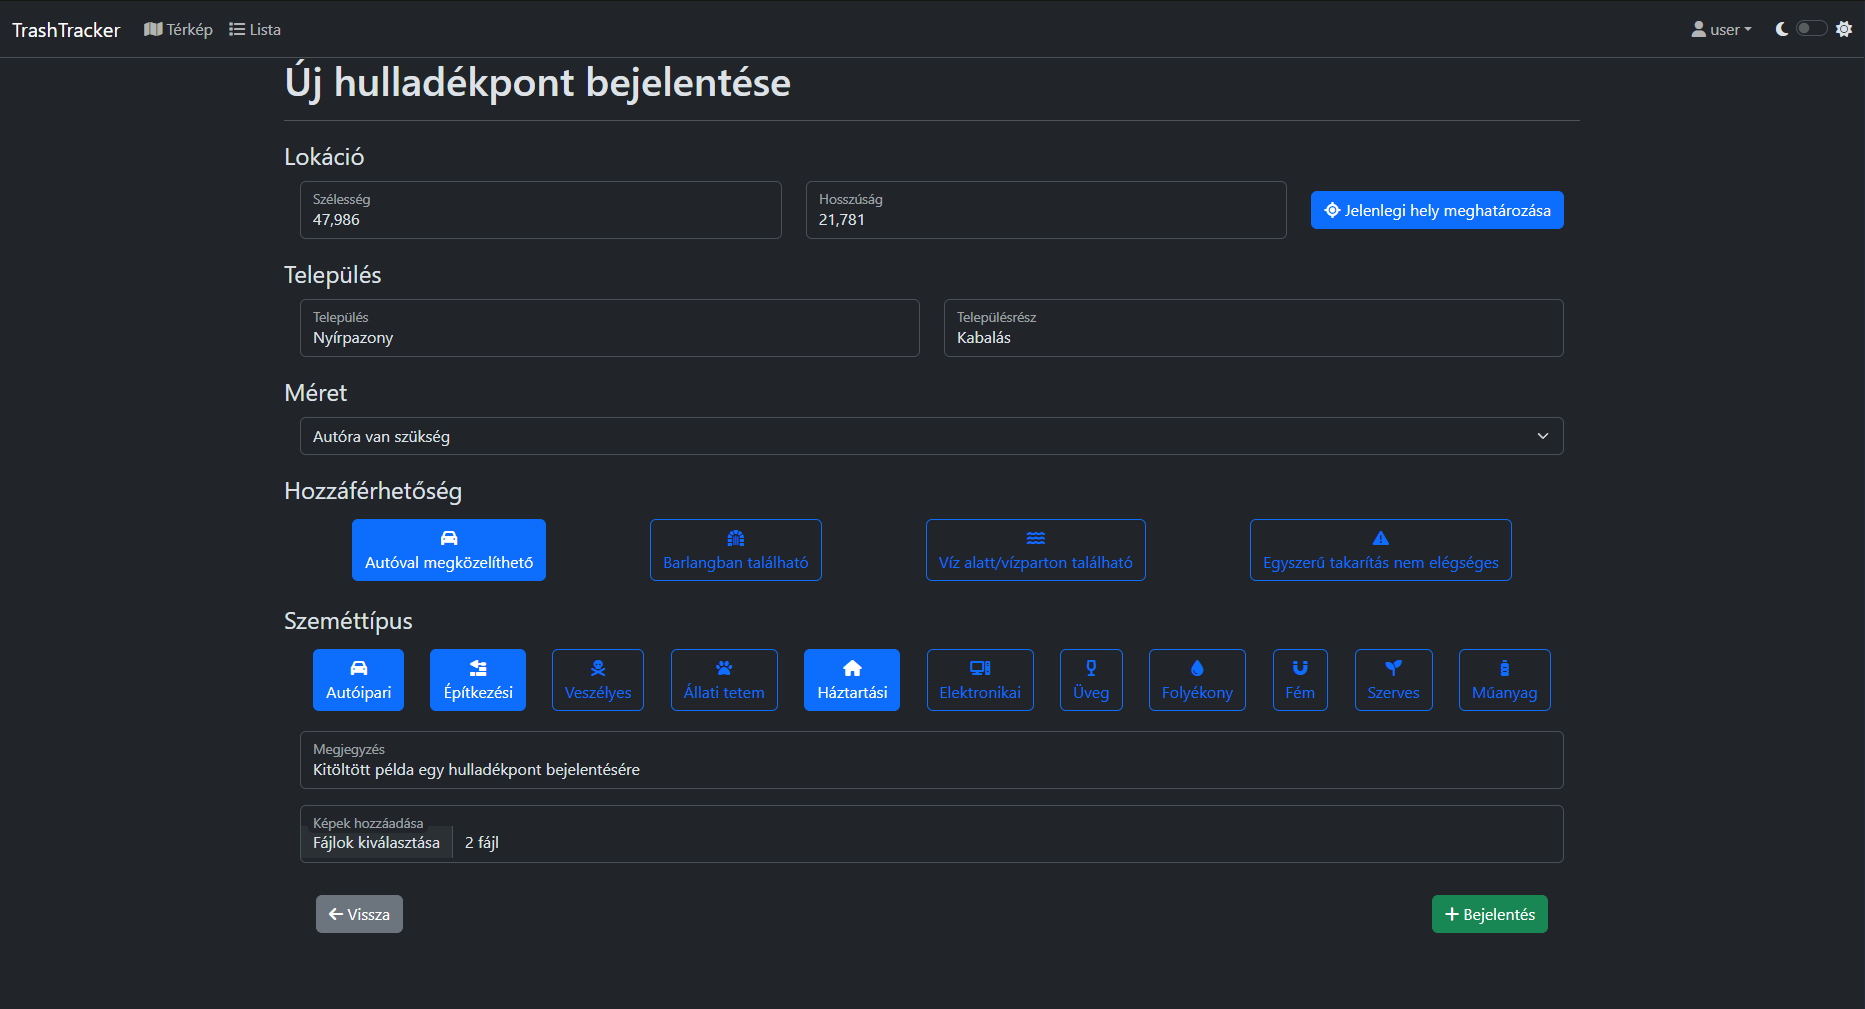
\includegraphics[width=0.7\textwidth]{trash_create}
	\caption{Szemétpont bejelentésének űrlapja}
	\label{fig:trash_create}
\end{figure}

\subsubsection{Hibaüzenetek}
\label{subsubsec:trash_create_errors}

Egy pont bejelentésekor egyedül a koordináták megadása kötelező, de erősen ajánlott további adatok leírása, illetve fénykép csatolása is. Ha a felhasználó nem ad meg egy kötelező adatot vagy beküldés előtt törli azt, akkor az űrlap egy "\textcolor{red}{<adat> megadása kötelező!}" hibaüzenettel jelzi azt az adott mező alatt. A koordinátákkal kapcsolatosan vannak triviális követelmények is, mely szerint nem lehet kevesebb, mint -180 és több, mint 180, mely megsértésekor egy "\textcolor{red}{A koordináta nem lehet kevesebb, mint -180° és több, mint 180°.}". Emellett az elfogadott formátum a tizedesvessző (tehát nem a -pont) használata. A megjegyzésbe bármit lehet írni, viszont biztonsági okokból az nem lehet több, mint 2000 karakter, mely túllépése esetén egy "\textcolor{red}{2000 karakternél nem lehet hosszabb a megjegyzés!}". A képekkel kapcsolatosan van a legtöbb technikai követelmény, melyek kizárólag fájlok, azon belül is kép, ahol csak ".jpg" (vagy ".jpeg"), illetve ".png" formátumúak lehetnek, amelyek nem léphetik túl az 1 MB méretet. Ezen pontok megsértésekor rendre "\textcolor{red}{Az objektum nem fájl!}", "\textcolor{red}{A fájl nem egy kép!}", "\textcolor{red}{Ez a kép formátuma nem támogatott! Támogatott formátumok: ".jpg", ".jpeg", ".png".}", illetve "\textcolor{red}{Ez a kép túl nagy! Maximális méret: 1024KB.}" hibaüzenetekkel találkozhat a felhasználó. \textbf{A bejelentés csak akkor véglegesedik, ha hiba nélkül sikerül megadni az adatokat!}

\subsection{Pont módosítása}

Egy már meglévő pont adatainak módosítására az azt részletező adatlap alján található "Módosítás", vagy a listanézet egyes soraiban található \faIcon{edit} ikonra kattintva érhető el. Az ezen az oldalon található űrlap hasonló, a pont létrehozáskor használtéhoz, a szemét állapotának lenyíló menüjét leszámítva, melynek megadása létrehozáskor még értelmetlen lenne. Emellett a meglevő képek felülírása helyett az itt megadottak (a hozzátartozó mező leírásához hűen) a ponthoz hozzáadásra kerülnek, a régieket megtartva.

\begin{figure}[H]
	\centering
	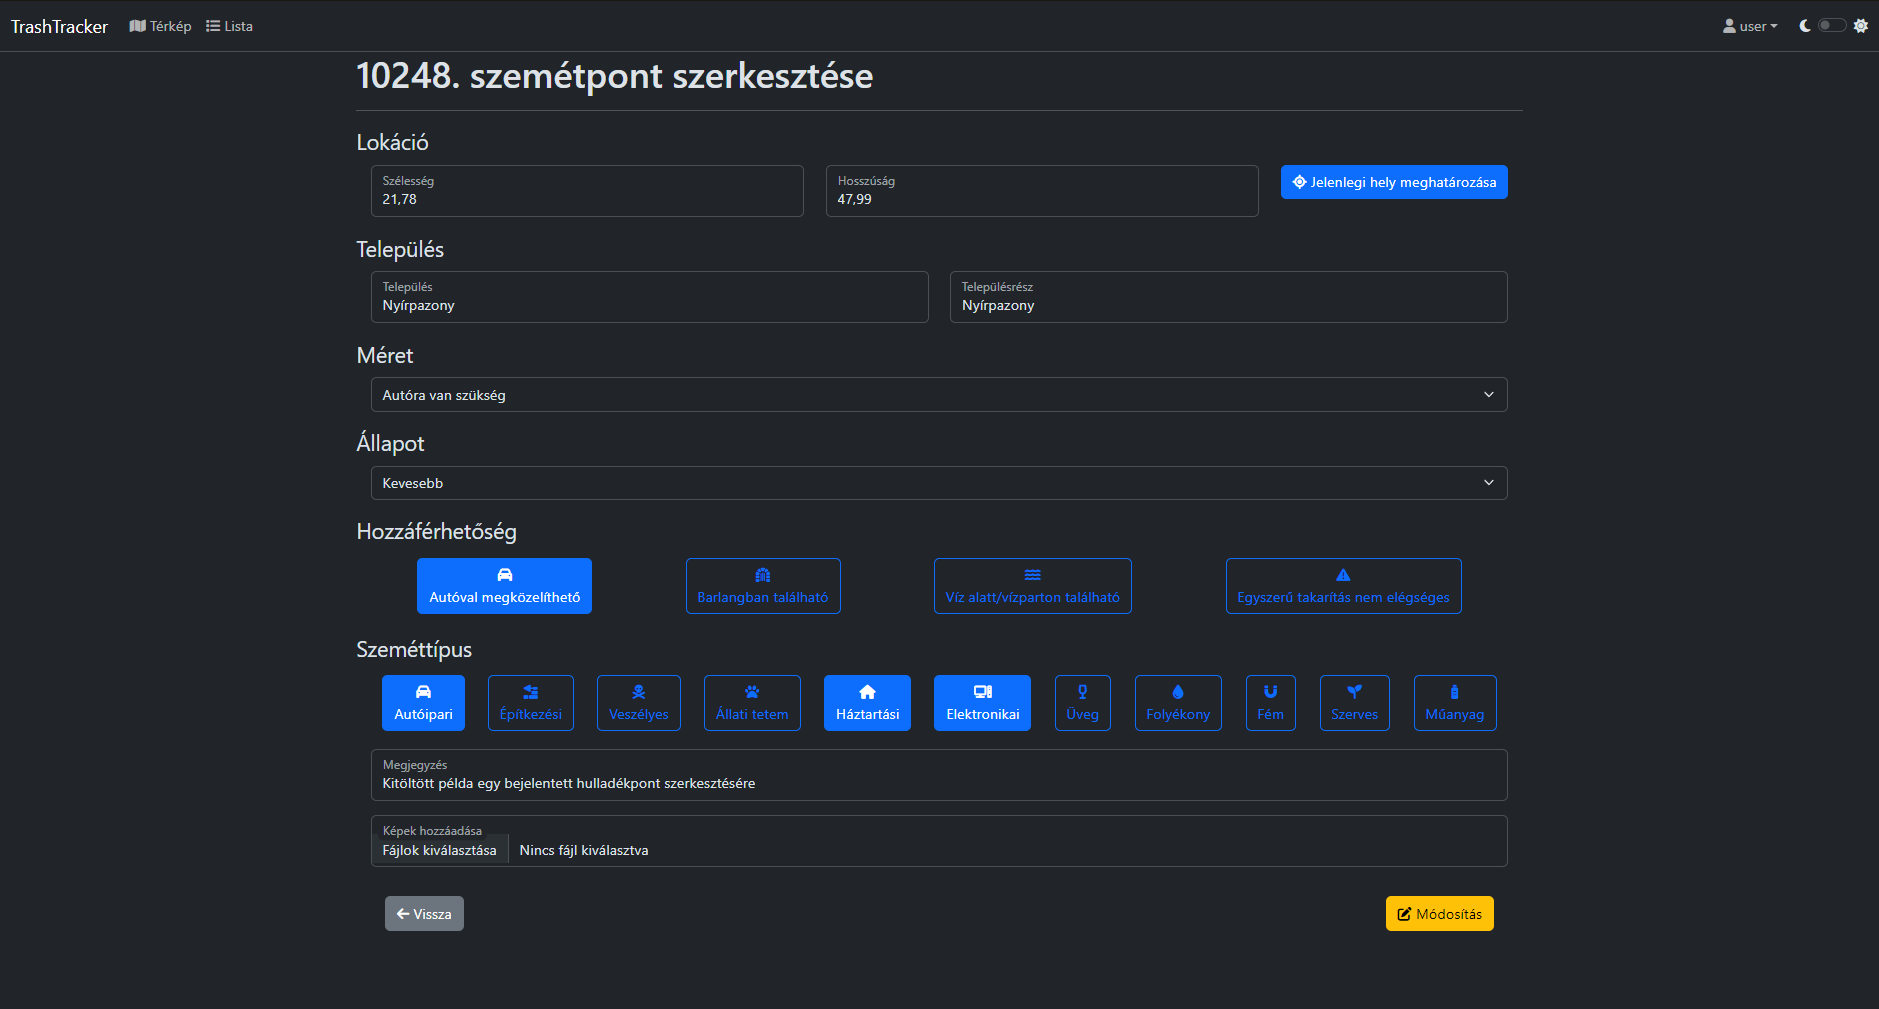
\includegraphics[width=0.7\textwidth]{trash_edit}
	\caption{Szemétpont módosításának űrlapja}
	\label{fig:trash_edit}
\end{figure}

\subsubsection{Hibaüzenetek}

Az itt megjelenő hibaüzenetek azonosak a \ref{subsubsec:trash_create_errors} bekezdésben tárgyaltakkal.

\subsection{Saját profil megtekintése}
\label{subsec:user_details}

A felhasználó regisztrálásával mindenki egy saját profil oldalra is szert tesz. A saját megtekintéséhez a navigációs sáv jobb oldalán, a felhasználónévre kattintva lenyíló menüben a "Saját profil" menüpontra nyomva van lehetőség.\\
Minden profiloldal fejlécében a bal oldalon a profilkép (ha van, ellenben egy "\textit{Nincs profilkép}" felirat), mellette pedig a felhasználó neve, illetve elérhetősége (e-mail címe) található. Ha a saját profilunk böngésszük, akkor az elérhetőségünk mellett találjuk a "Profil szerkesztése" gombot, mely értelemszerűen annak a szerkesztését segítő űrlapra navigál. Ez alatt az adott felhasználó által bejelentett pontok listanézete található, amely használata azonos a \ref{subsec:trash_index} bekezdésben tárgyaltakkal, a szűrési lehetőségeket leszámítva.

\begin{figure}[H]
	\centering
	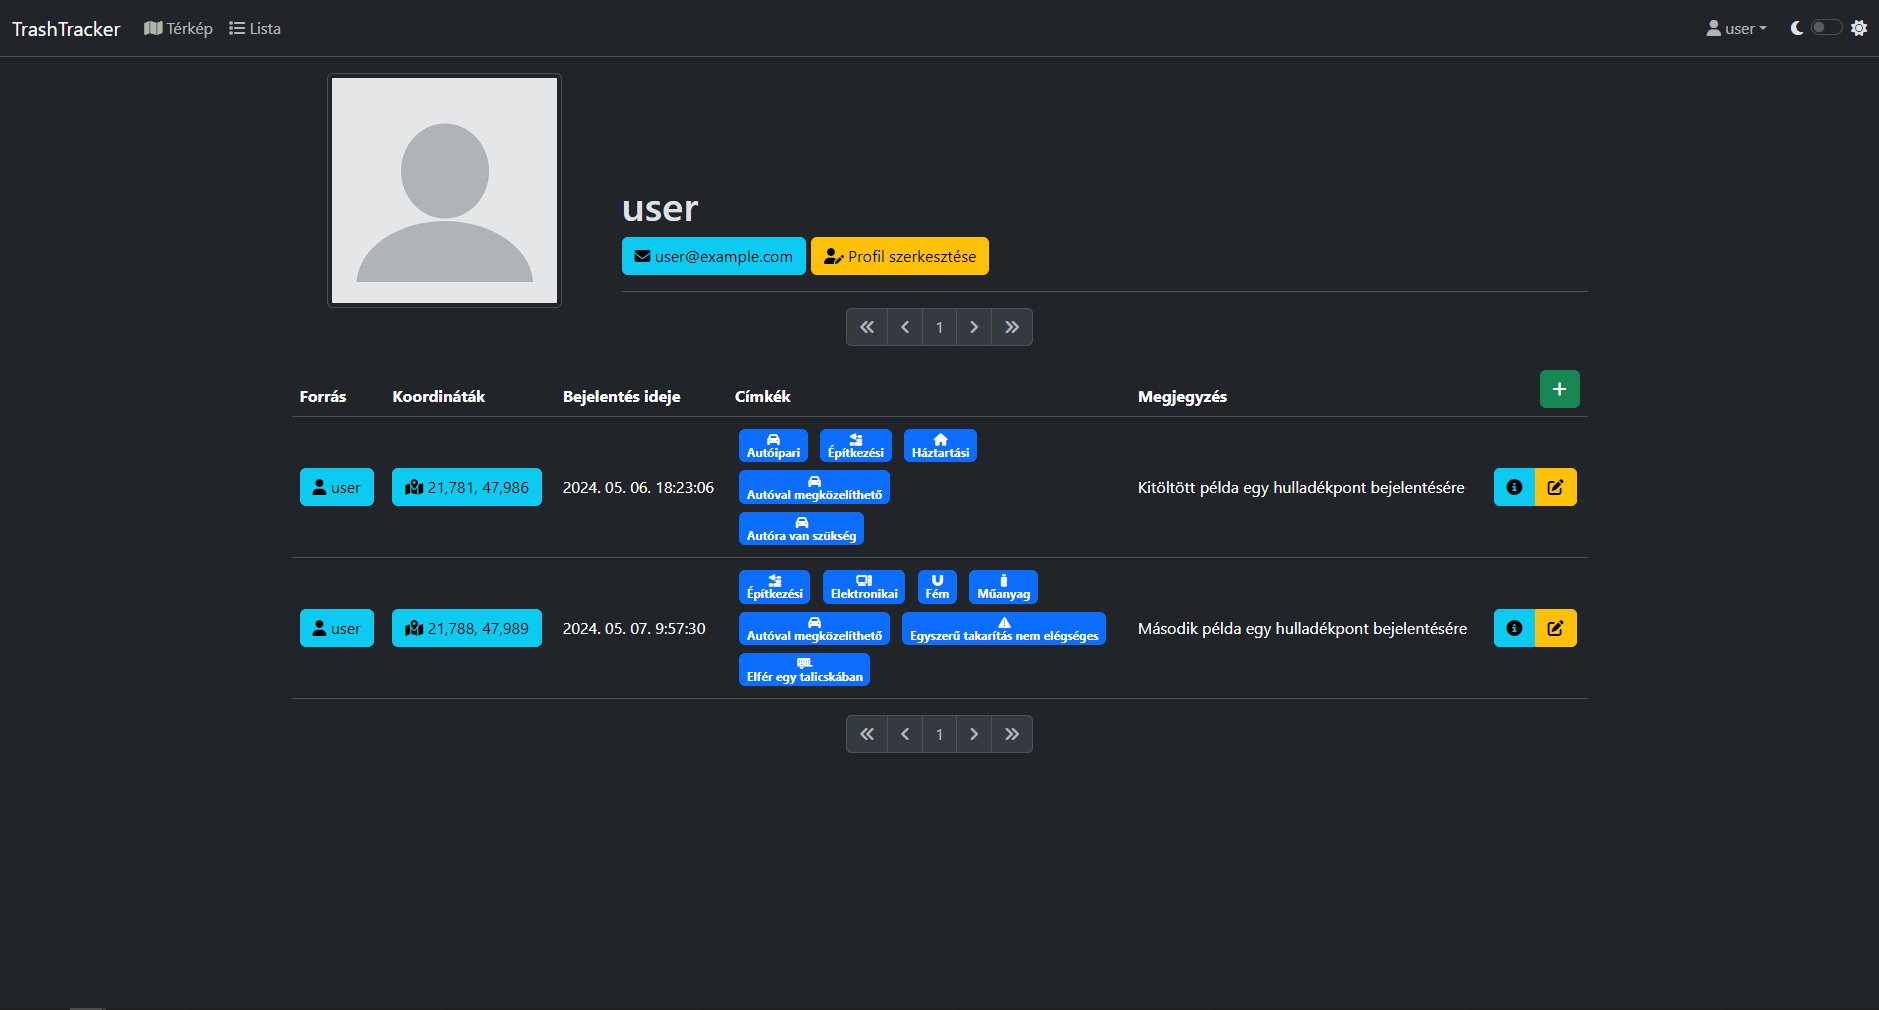
\includegraphics[width=0.7\textwidth]{user_details}
	\caption{Példa egy felhasználói profilra}
	\label{fig:user_details}
\end{figure}

\subsubsection{Más felhasználó profiljának megtekintése}

Egyszerű felhasználói fiókkal nincs lehetőség további felhasználók "felderítésére", csak az általuk bejelentett pontokon levő hivatkozásokkal. Mind a pontok listanézetében (\ref{subsec:trash_index} bekezdés), illetve azok adatlapján (\ref{subsec:trash_details} bekezdés) találhatóak ezek, ahol az adott fejezetekben tárgyaltak szerinti \faIcon{user} ikonnal ellátott gombokra kattintva van lehetőség.

\subsection{Saját profil szerkesztése}
\label{subsec:user_edit}

A saját profil megtekintésekor (\ref{subsec:user_details} bekezdés) a "Profil szerkesztése" gombra kattintva van lehetőség a felhasználónév, e-mail cím és profilkép módosítására. Ehhez is egy űrlap áll a rendelkezésre, mely a gombra kattintáskor jelenik meg, az előbb említett adatok mezőivel. Az alján található "Módosítás"-ra nyomva azok a mezők, melyek tartalmaznak adatot, és ha tartalmaznak akkor újat, módosulni fognak, feltéve ha hiba nélkül megy végbe az.

\begin{figure}[H]
	\centering
	\subcaptionbox{Profil szerkesztésének űrlapja}{
		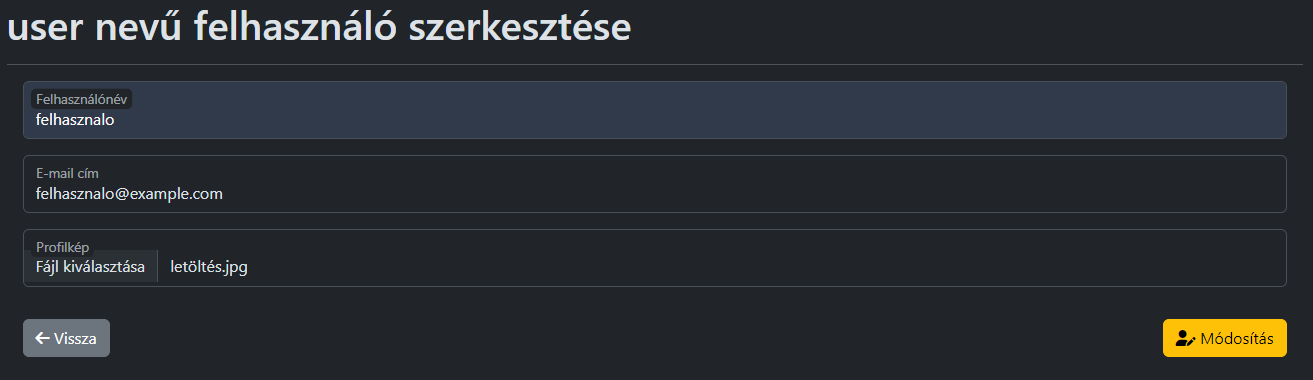
\includegraphics[width=0.4\textwidth]{user_edit}}
	\hspace{5pt}
	\subcaptionbox{Szerkesztés utáni profiloldal}{
		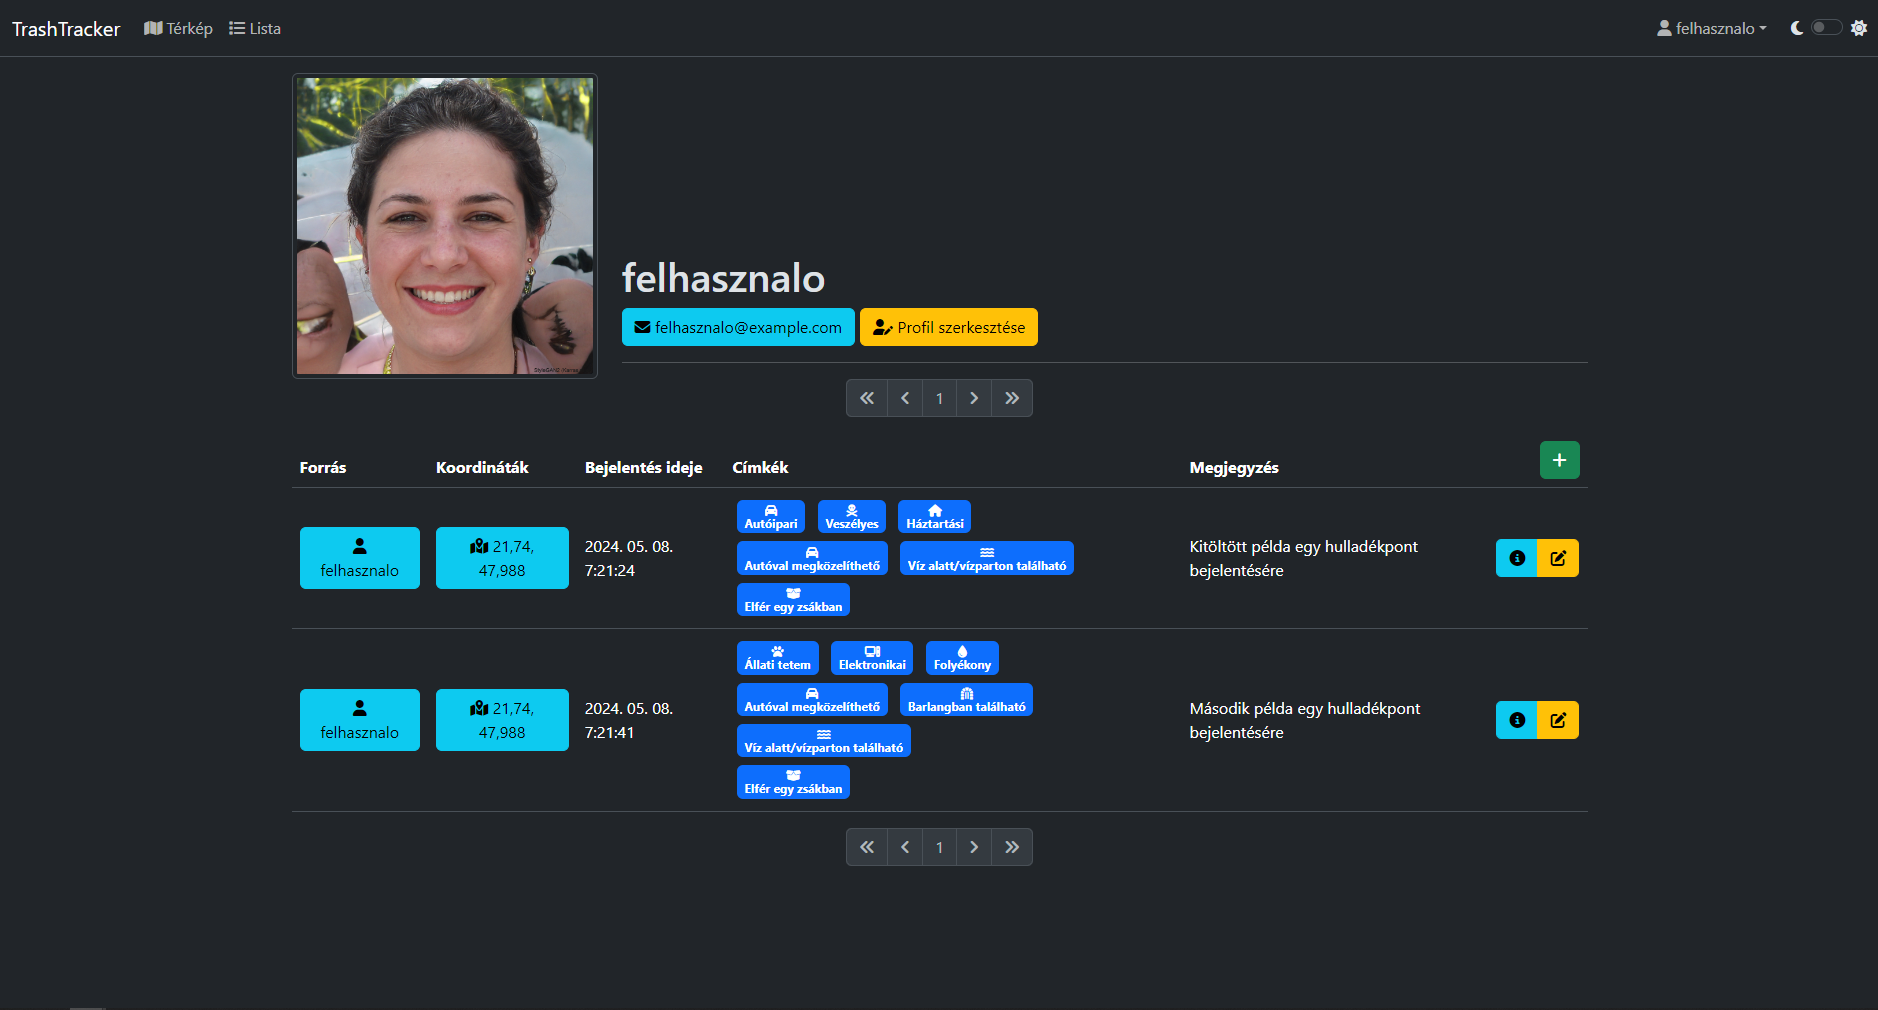
\includegraphics[width=0.55\linewidth]{user_details_edited}}
	\caption{Profil szerkesztése és annak eredménye}
	\label{fig:user_edit}
\end{figure}

\subsubsection{Hibaüzenetek}

Az űrlap elküldésekor van lehetőség, hogy sikeres módosítás helyett hibaüzenetet kapunk (ilyenkor az adatok nem módosulnak  még). Mivel minden felhasználónévnek és e-mail címnek egyedinek kell lennie, így ha azok mégsem lennének a módosítás után, 
akkor rendre "\textcolor{red}{A felhasználónév már foglalt!}", illetve "\textcolor{red}{Az e-mail cím már foglalt!}" üzenetekkel találkozhat a felhasználó. Emellett ez e-mail címnek érvényes formátumúnak kell lennie, és a profilképnek is meg kell felelnie a regisztráláskor definiáltakkal, mely a \ref{subsubsec:user_register_errors} bekezdésben van tárgyalva.

\begin{figure}[H]
	\centering
	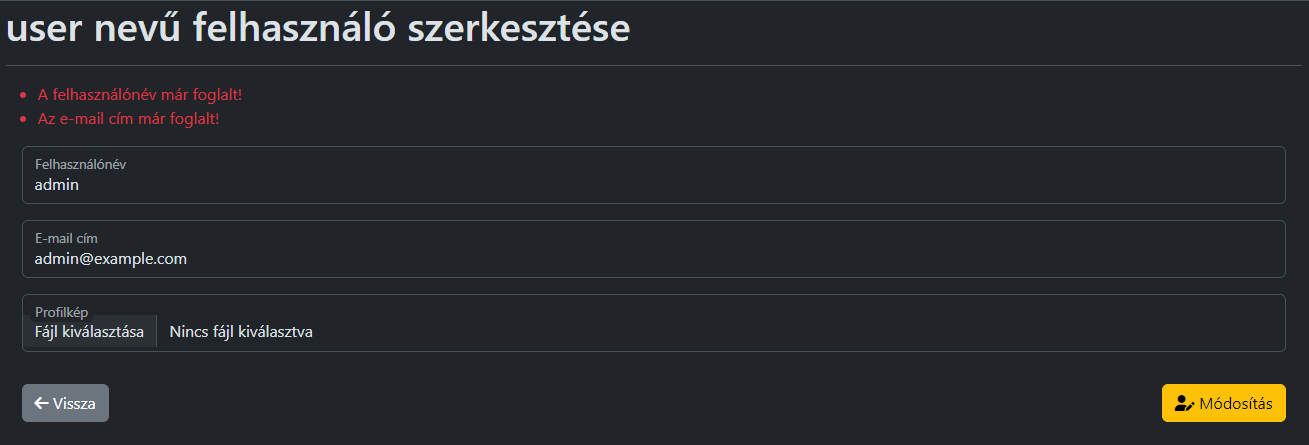
\includegraphics[width=0.7\textwidth]{user_edit_errors}
	\caption{Profil szerkesztésének űrlapja}
	\label{fig:user_edit_errors}
\end{figure}

\section{Funkciók moderátorként}

A moderátor szintű felhasználói fiókok mindenre jogosultak, mint az egyszerű felhasználók, viszont képesek bejelentett pontok törlésére, ezzel az esetleges "spam" moderálására.

\begin{figure}[H]
	\centering
	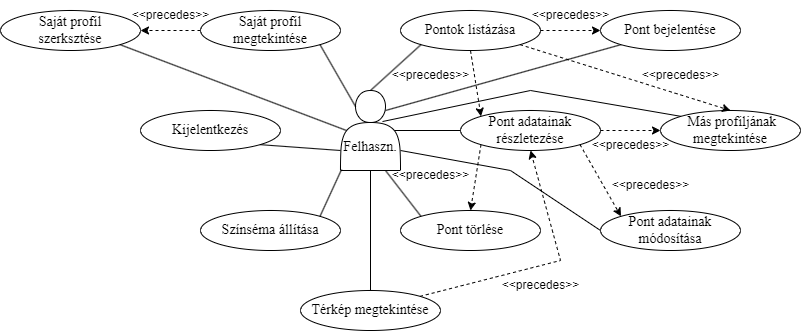
\includegraphics[width=1.0\textwidth]{usecase_moderator}
	\caption{Felhasználói esetek moderátorként}
	\label{fig:usecase_moderator}
\end{figure}

\subsection{Pont törlése}
\label{subsec:trash_delete}

Egy pont törlésére azok listanézetéből a \faIcon{trash} ikonra vagy annak adatlapján található "Törlés" gombra kattintva van lehetőség. A "balesetek" elkerülése érdekében először egy megerősítő oldalra navigál, ahol "Vissza" és "Törlés" opciók közül lehet választani, melyek rendre az előző oldalra navigálnak (törlés nélkül), illetve véglegesen törlik az adott pontot.

\begin{figure}[H]
	\centering
	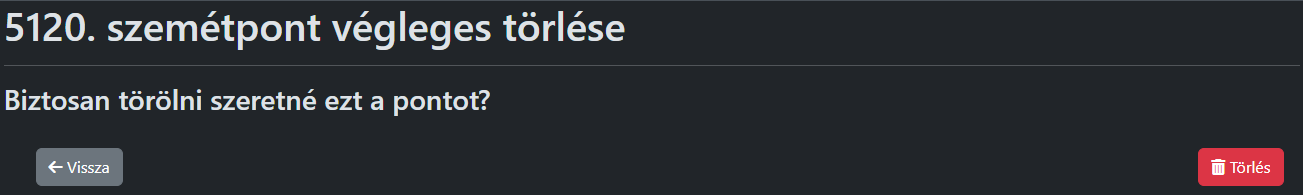
\includegraphics[width=0.7\textwidth]{trash_delete}
	\caption{Pont törlésének megerősítő űrlapja}
	\label{fig:trash_delete}
\end{figure}

\section{Funkciók adminisztrátorként}

Az adminisztrátori szintű fiókok mindenre jogosultak, tehát az előbb említett funkciók mellett képes a felhasználói fiókok listázására, azok módosítására, illetve törlésére is.

\subsection{Felület áttekintése}
\label{subsec:nav_admin}

A \ref{subsec:nav_guest} bekezdésben tárgyalt navigációs felületen adminisztrátorként egy újabb hivatkozás válik elérhetővé "Felhasználók" névvel. Erre való kattintással elérhető az összes felhasználói fiók listázása.

\subsection{Felhasználói fiókok listázása}

Ez a felület a \ref{subsec:nav_admin} bekezdésben tárgyalt navigációs sávban található menüponttal érhető el, ha adminisztrátori szintű fiókkal van a felhasználó bejelentkezve. Kezelése hasonló a \ref{subsec:trash_index} bekezdésben tárgyalt szemétpontok listanézetével. A lista tetején ugyanúgy megtalálható a már megismert szűrő beállítások, ahol felhasználó vagy e-mail cím alapján lehet keresni, illetve a találatok lapszámát állítani. Ez alatt található a lista, ahol minden fiók felhasználónevét, e-mail címét és regisztrálási idejét (ha alapértelmezetten generált fiók, akkor az érték "0001. 01. 01. 0:00:00") lehet megtalálni, regisztrálás ideje szerint sorrendben (azaz a legfrissebb fiókok vannak előbb). Emellett minden rekord végén található három gomb, mely rendre az adott fiókhoz tartozó profil megtekintésére, -szerkesztésére és törlésére szolgál.

\begin{figure}[H]
	\centering
	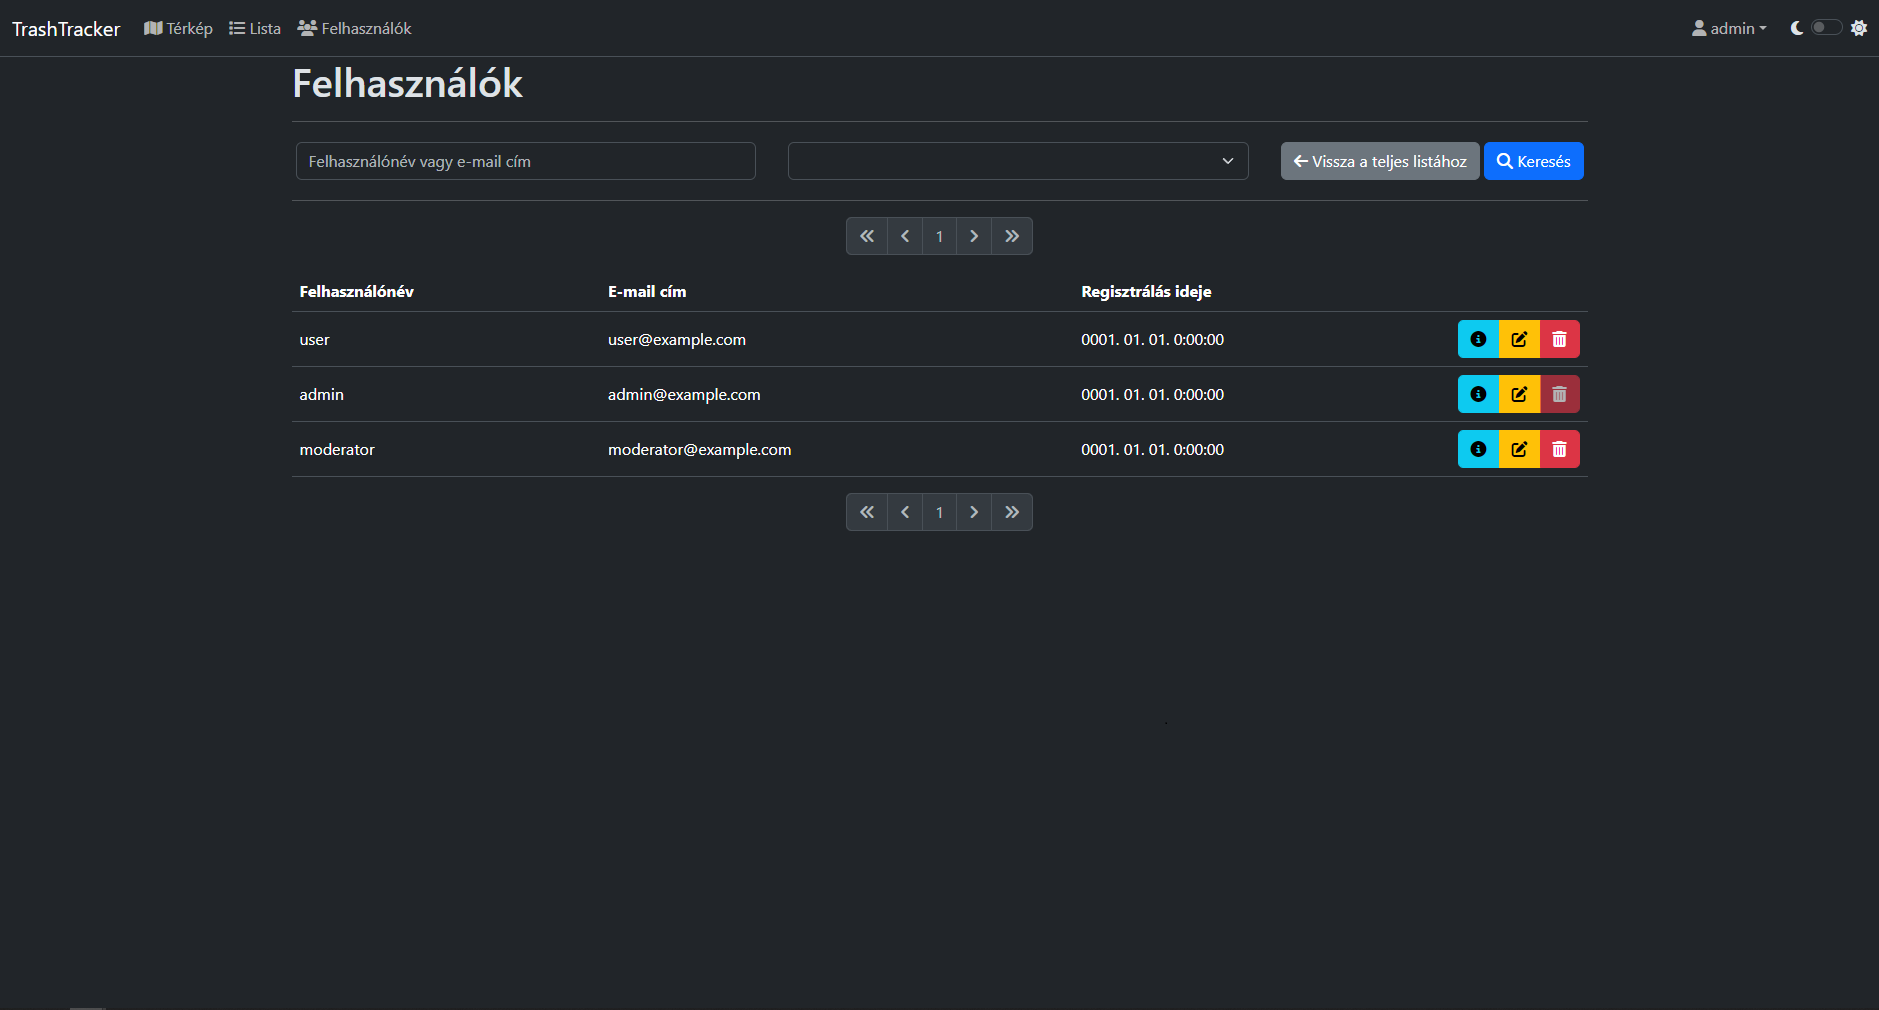
\includegraphics[width=0.7\textwidth]{user_index}
	\caption{Felhasználói fiókok listanézetének felülete}
	\label{fig:user_index}
\end{figure}

\subsection{Felhasználói fiókok módosítása}

A módosítás űrlapja hasonló, a \ref{subsec:user_edit} bekezdésben tárgyaltakkal, viszont itt lehetőség van egy adott felhasználói fiók hozzáférési szintjét állítani egy lenyíló lista segítségével. Biztonsági okok miatt a saját felhasználó jogosultsági köre nem módosítható, az erre való lista nem jelenik meg az űrlapon.

\begin{figure}[H]
	\centering
	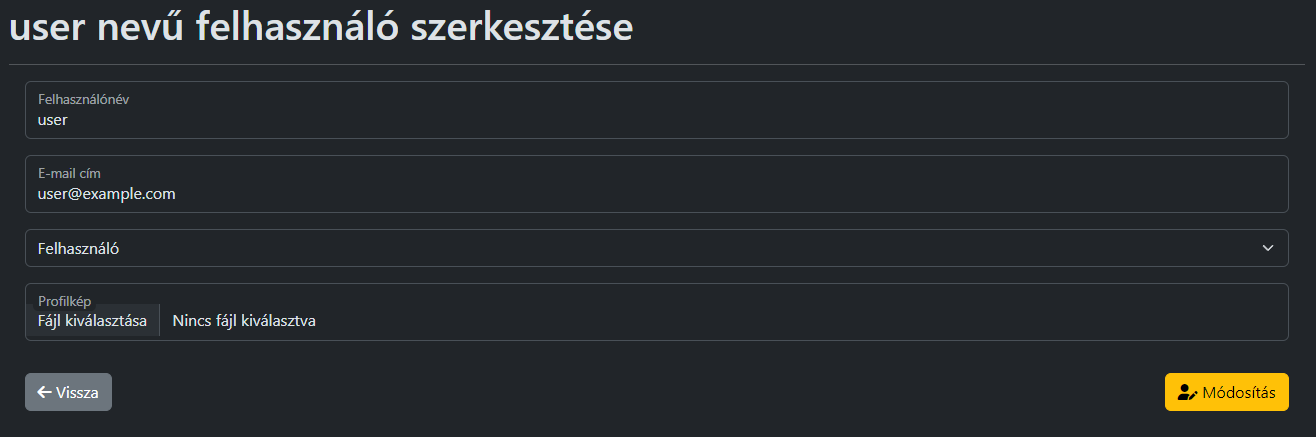
\includegraphics[width=0.7\textwidth]{user_edit_admin}
	\caption{Felhasználói fiókok szerkesztési űrlapja adminisztrátorként}
	\label{fig:user_edit_admin}
\end{figure}

\subsection{Felhasználói fiókok törlése}

A törlés folyamata is megegyezik a \ref{subsec:trash_delete} bekezdésben tárgyalt pontéval. Biztonsági okok miatt, a saját felhasználót törölni nem lehet, a listában is az erre mutató gombhivatkozás nem kattintható.

\begin{figure}[H]
	\centering
	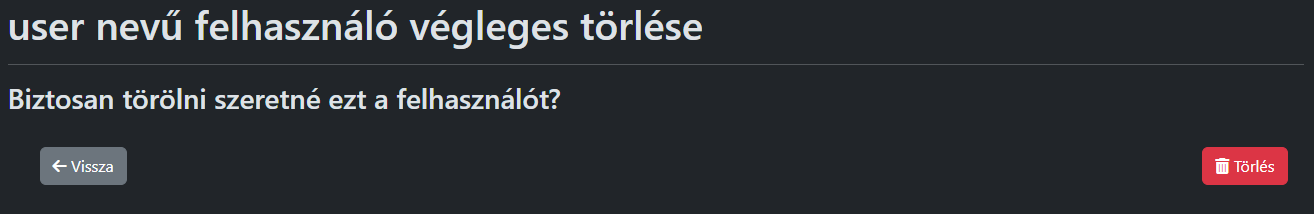
\includegraphics[width=0.7\textwidth]{user_delete}
	\caption{Felhasználói fiókok törlésének megerősítő űrlapja}
	\label{fig:user_delete}
\end{figure}